\begin{frame}{Fonctionnement de la librairie \texttt{keybert}}
\begin{enumerate}[<+->]
\item entrée : un document
\item tokénisation du document en mots/phrases-clés candidates
\item génération des plongements du document et des mots/phrases-clés
\item calcul de la similarité cosinus document : mots/phrases-clés
\end{enumerate}
\begin{figure}
    \centering
    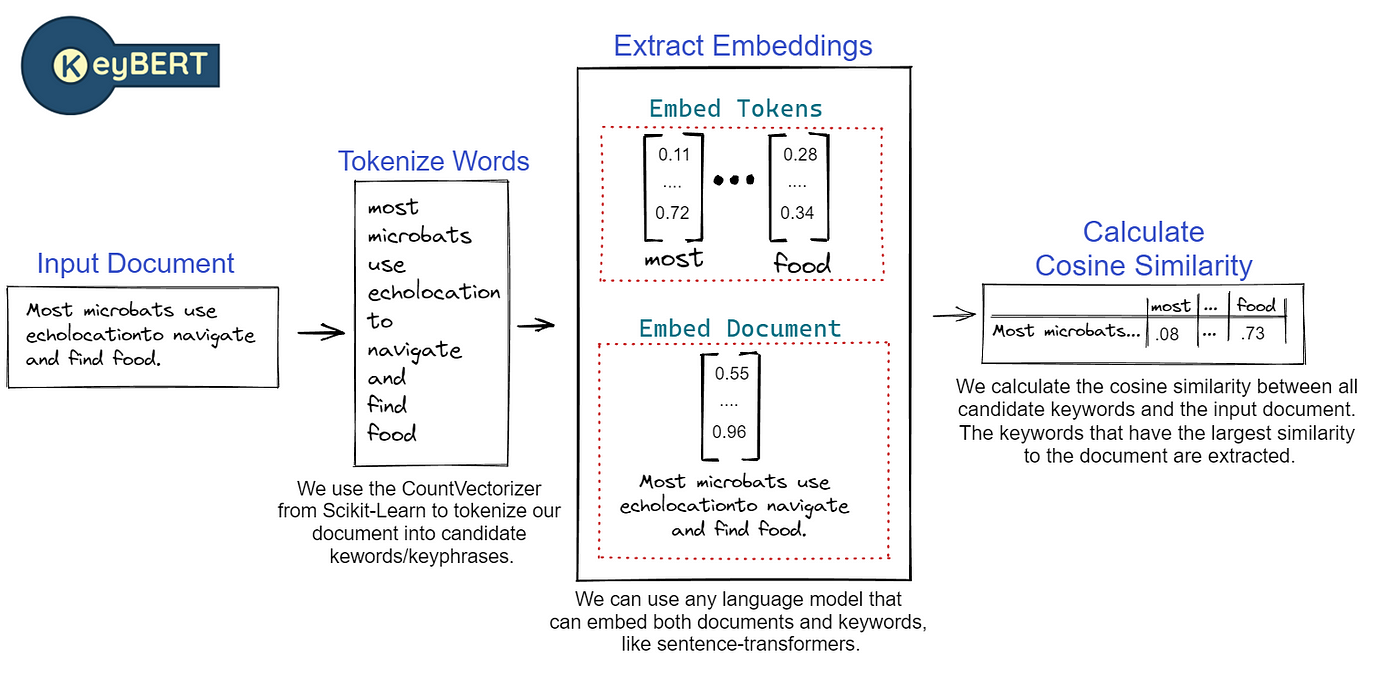
\includegraphics[width=80mm,scale=0.5]{pic/keybert.png}
    \caption{\textit{Pipeline} de la méthode \texttt{keybert} \citep{grootendorst2020keybert}.}
    \label{fig:enter-label}
\end{figure}
\end{frame}

\begin{frame}{Liste des phrases-clés extraites avec \texttt{keybert}}
\begin{table}
\small
\begin{tabular}{l|r}
\rowcolor[HTML]{FFCCC9} 
\textsc{\textbf{Phrase-clé}} & \cellcolor[HTML]{DAE8FC}\textsc{\textbf{Score}} \\ \hline
postérieure cordon postérieur & 0.5078 \\
scientifique les planches &  0.4944 \\
antérieure corne postérieure & 0.486 \\
cervico dorsale & 0.465 \\
cervicale la figure & 0.4311 \\
faisceau postérieur tumeur & 0.4276 \\
avoisinante cellule ganglionnaire & 0.3836 \\
lcucocythcs substance granuleuse & 0.3474 \\
moëlle épinière 45 & 0.3381 \\
complètement détruite & 0.334 \\
\end{tabular}
\caption{Liste des dix phrases-clés les plus pertinentes selon \texttt{keybert}.}
\end{table}
\end{frame}

